\subsection{Stability}

Stability of open or even closed loop systems is an important concept in control systems. An open loop system is stable if the output of the system remains bounded for a bounded input. In other words, if the input to the system is a step function, the output of the system will reach a steady state value and not diverge to infinity. The stability of a system can be analyzed using the characteristic equation of the system which was shown in the solution to multiple differential equations. The astute reader will have also noticed that the denominator of the transfer function is identical to the characteristic equation. The roots of the characteristic equation are often called the poles of the system and can be used interchangeably. Thus, the benefit of a transfer function is that stability can be ascertained immediately by looking at the denominator of the transfer function. In the Chapter on feedback control it will be shown that control systems in the laplace domain can be applied by simply multiplying different control systems and examining the resulting closed loop transfer function for stability. When designing controllers in the time domain it is almost impossible to gaurantee closed loop stability. However, with transfer functions, after a bit of algebraic manipulation stability can be ascertained. 

So what do the poles or roots of the characteristic equation tell you? Remember that the general soltion to a differential equation is $q(t) = Ae^{st}$. The value of $s$, the roots, the poles, tell whether the system will oscillate, decay or extend off to infinity. The location of the poles in the complex plane determines the stability of the system. If all poles have negative real parts, the system is stable. This would results in an equation like $e^{-st}$ where that term tends to 0 as $t \rightarrow \infty$. If any pole has a positive real part, the system is unstable. If any pole has a real part equal to zero, the system is marginally stable. Marginal stability is defined as a system that neither grows nor decays but rather oscillates indefinitely or increases but not faster than a linear term. This would result in an equation like $e^{j\omega t}$  or $f_0 t$ which is a sine/cosine function or linear term. The imaginary part of the pole determines the frequency of oscillation. The real part of the pole determines the rate of decay or growth. A pole with a large negative real part will result in a fast decay while a pole with a small negative real part will result in a slow decay. A pole with a large positive real part will result in a fast growth while a pole with a small positive real part will result in a slow growth. The sections that follow examine the transfer functions of the systems examined earlier and determine their stability. The equations below summarize the stability criteria.
\begin{itemize}
    \item {\bf Stable}: All poles have negative real parts. $Re(s) < 0$
    \item {\bf Unstable}: Any pole has a positive real part. $Re(s) > 0$
    \item {\bf Marginally Stable}: Any pole has a real part equal to zero. $Re(s) = 0$
\end{itemize}
Note that for the sections that follow code has been added to all the python scripts in the Time Response section such as \href{https://github.com/cmontalvo251/Python/blob/master/controls/satellite.py}{satellite.py} or \href{https://github.com/cmontalvo251/Python/blob/master/controls/mass_spring_damper.py}{mass\_spring\_damper.py}. The code added plots the poles of each system on a real-imaginary plot to visually show the stability of each system. For clarity on the code, the Figure below shows the relevant function used to plot the poles of each system which again has been added to Github.
\begin{figure}[H]
\centering
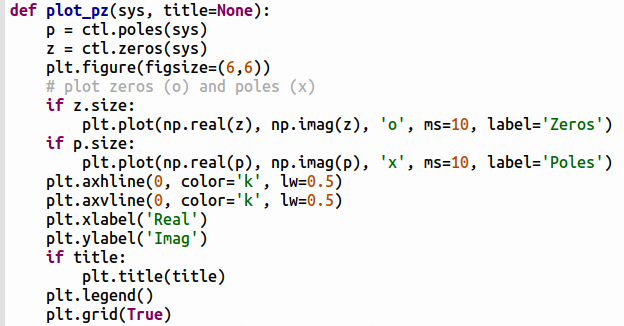
\includegraphics[width=0.8\linewidth]{Figures/pole_zero_code.png}
\caption{Pole-Zero Plotting Code}
\label{f:pole_zero_code}
\end{figure}

\subsubsection{Position and Velocity of a Car}

As derived earlier the transfer function for the position of the car is given as 
\begin{equation}
    \frac{X(s)}{F(s)}= G(s) = \frac{\sigma}{s(s+\sigma)}
\end{equation}
recall also that the time domain solution to this system due to a step function was given as 
\begin{equation}
    x(t) = f_0 t - \frac{f_0}{\sigma} (1 - e^{-\sigma t})
\end{equation}
Plotted in the time domain the system accelerated and then attained a constant velocity. The poles of the system are located at $s=0$ and $s=-\sigma$. The pole at $s=-\sigma$ has a negative real part and thus is stable. This is due to the $1/(s+\sigma)$ term which translates to the $e^{-\sigma t}$ term in the time domain. The pole at $s=0$ has a real part equal to zero and thus is marginally stable as given by the $1/s$ term in the laplace domain and the $f_0 t$ term in the time domain. The marginal stability is apparent because the position of the car will continue to increase linearly over time due to the constant velocity. However, the velocity of the car will reach a steady state value and not diverge to infinity. Thus, the system is considered stable for velocity. Remember the transfer function for velocity is found by simply multiplying the position transfer function by $s$ or taking the derivative in the time domain. The transfer function for velocity is given as
\begin{equation}
    \frac{V(s)}{F(s)}= G(s) = \frac{\sigma}{s+\sigma}
\end{equation}
while the time domain solution to this system due to a step function was given as
\begin{equation}
    v(t) = f_0 (1 - e^{-\sigma t})
\end{equation}
The pole of the velocity system is located at $s=-\sigma$ again from the $1/(s+\sigma)$ term in the laplace domain and the $e^{-\sigma t}$ term in the time domain. The pole has a negative real part and thus is stable. This is because the velocity of the car will reach a steady state value and not diverge to infinity. Examining both systems in the laplace domain is much easier than examining the time domain solutions because you can simply look at the poles of the transfer function. It is also beneficial to plot the poles of the system on a real-imaginary plot as shown in Figure \ref{f:car_poles}.
\begin{figure}[H]
\centering
\begin{subfigure}[b]{0.48\textwidth}
\centering
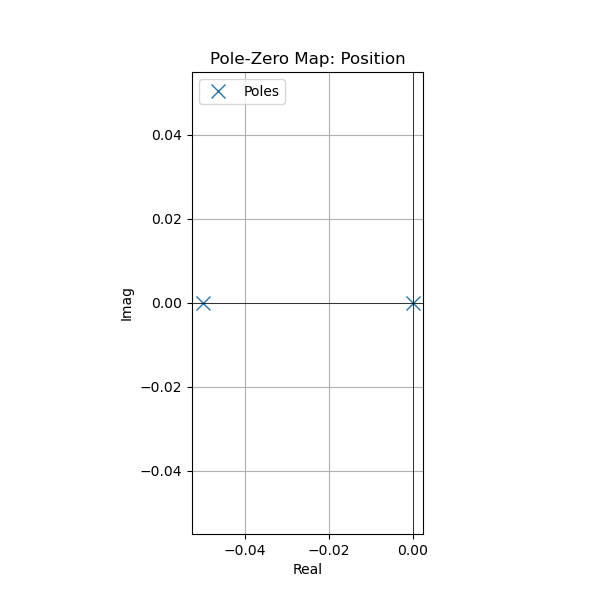
\includegraphics[width=\linewidth]{Figures/car_position_poles.png}
\end{subfigure}
\hfill
\begin{subfigure}[b]{0.48\textwidth}
\centering
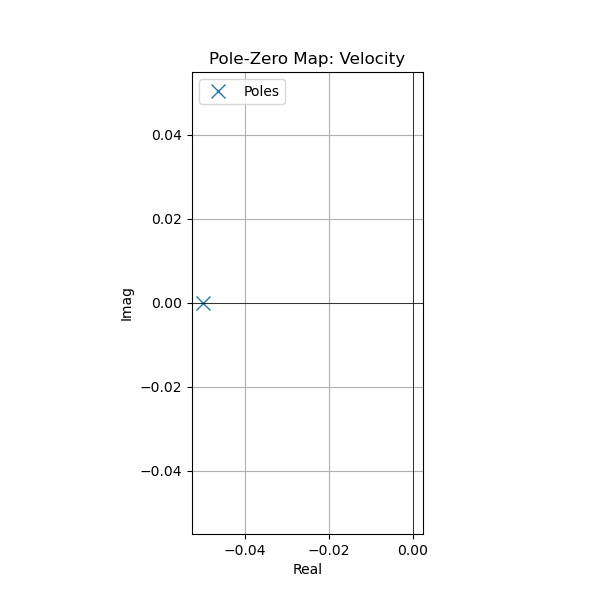
\includegraphics[width=\linewidth]{Figures/car_velocity_poles.png}
\end{subfigure}
\caption{Poles of Car System (Position (left) and Velocity (right))}
\label{f:car_poles}
\end{figure}
Notice that the poles of the position system are located at $s=0$ and $s=-\sigma$ while the pole of the velocity system is located at $s=-\sigma$. The position system has one marginally stable pole and one stable pole while the velocity system has one stable pole. Thus, the position system is marginally stable while the velocity system is stable. Remember if at least one pole is marginally stable and none are unstable the system is considered marginally stable. If all poles are stable the system is considered stable.

\subsubsection{Position of a Mass Spring Damper}

As derived earlier the transfer function for the position of the mass spring damper is given as 
\begin{equation}
    \frac{X(s)}{F(s)}= G(s) = \frac{{\omega_n}^2}{s^2 + 2\zeta \omega_n s + {\omega_n}^2}
\end{equation}
recall also that the time domain solution to this system due to a step function was given as 
\begin{equation}
    x(t) = f_0 \left( 1 - e^{-\zeta \omega_n t} \left( \cos(\omega_d t) + \frac{\zeta}{\sqrt{1-\zeta^2}} \sin(\omega_d t) \right) \right)
\end{equation}
for the underdamped case. Plotted in the time domain the system oscillated and then attained a steady state value. The poles of the system are located at 
\begin{equation}
    s = -\zeta \omega_n \pm j \omega_n \sqrt{1-\zeta^2}
\end{equation}
The real part of the poles is $-\zeta \omega_n$ which is negative for all positive values of $\zeta$ and $\omega_n$. Thus, the system is stable for all positive values of $\zeta$ and $\omega_n$. Examining the system in the laplace domain is much easier than examining the time domain solutions because you can simply look at the poles of the transfer function. It is also beneficial to plot the poles of the system on a real-imaginary plot as shown in Figure \ref{f:mass_spring_damper_poles}.
\begin{figure}[H]
\centering
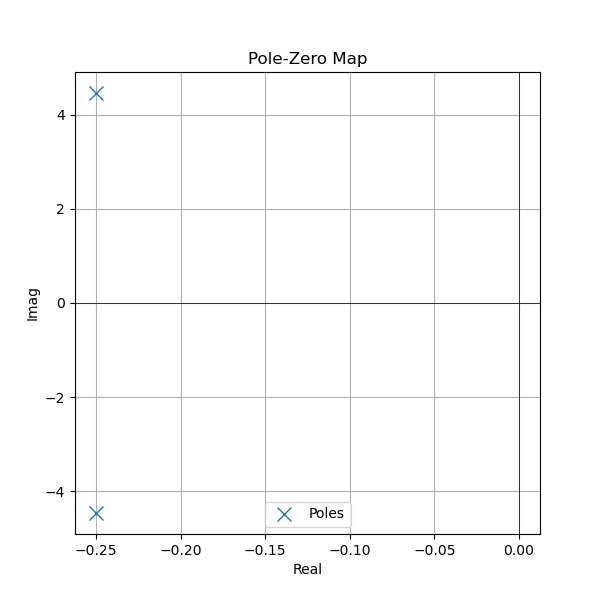
\includegraphics[width=0.6\linewidth]{Figures/mass_spring_damper_poles.png}
\caption{Poles of Mass Spring Damper System}
\label{f:mass_spring_damper_poles}
\end{figure}
Notice that the poles of the mass spring damper system are located in the left half of the complex plane. The real part of the poles is negative and thus the system is stable. The imaginary part of the poles determines the frequency of oscillation while the real part of the poles determines the rate of decay. The further left the poles are located in the complex plane, the faster the system will decay to its steady state value. Thus again the transfer function shows it's usefuleness in determining the stability of a system as well as whether it oscillates or not. In this case the system is stable (left half plane) and oscillatory (imaginary part non-zero).

\subsubsection{Attitude Dynamics of a Satellite or Quadcopter}

As derived earlier, the transfer function of this system is given as $\frac{\Theta(s)}{F(s)}= G(s) = \frac{2d}{Js^2}$. The poles of the system are located at $s=0$ and $s=0$. Both poles have real parts equal to zero and thus the system is marginally stable because they are on the y-axis of the real-imaginary plane. Physically, this marginal stability is because the angle of the satellite/quadcopter will continue to increase quadratically over time due to the constant angular acceleration from a constant force from the propellor/thrusters. The marginal stability can be seen in the time domain with the system increasing as $t^2$. However, examining the system in the laplace domain is much easier than examining the time domain solutions because you can simply look at the poles of the transfer function. Again, it is beneficial to plot the poles of the system on a real-imaginary plot as shown in Figure \ref{f:satellite_poles}.
\begin{figure}[H]
\centering
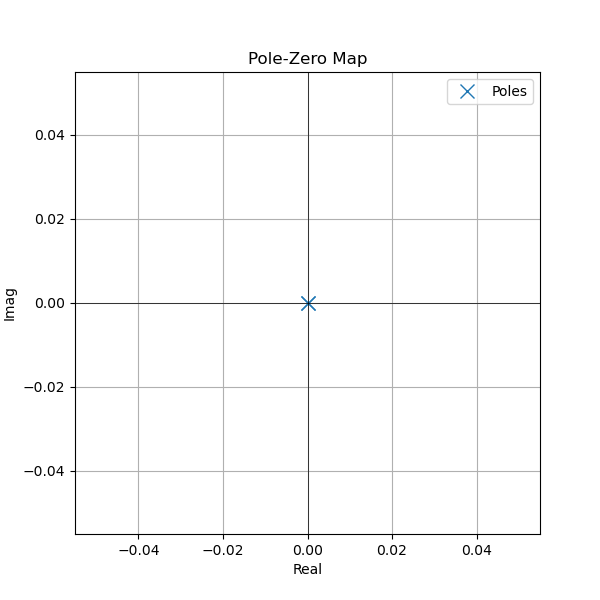
\includegraphics[width=0.4\linewidth]{Figures/satellite_poles.png}
\caption{Poles of Satellite/Quadcopter System}
\label{f:satellite_poles}
\end{figure}
Notice that the poles of the satellite/quadcopter system are located at $s=0$ and $s=0$. Both poles have real parts equal to zero and thus the system is marginally stable and increases quadratically over time. A single pole at zero would increase linearly but two poles at the origin increases quadratically.

\subsubsection{Pitch Dynamics of an Aircraft}

\subsubsection{Pitch Dynamics of a Rocket}

\subsubsection{Angle of an Inverted Pendulum}
